\documentclass{beamer}
\usetheme[pageofpages=of,% String used between the current page and the
                         % total page count.
          bullet=circle,% Use circles instead of squares for bullets.
          titleline=true,% Show a line below the frame title.
          alternativetitlepage=true,% Use the fancy title page.
       %   titlepagelogo=logo-polito,% Logo for the first page.
       %   watermark=watermark-polito,% Watermark used in every page.
       %   watermarkheight=100px,% Height of the watermark.
       %   watermarkheightmult=4,% The watermark image is 4 times bigger
                                % than watermarkheight.
          ]{Torino}

\setbeamertemplate{footline}{
  \begin{beamercolorbox}[wd=\paperwidth,ht=1ex,dp=1ex]{footline}
    \vspace{5pt} \hspace{1em} \insertframenumber/\inserttotalframenumber
  \end{beamercolorbox}
}

\author{Brendon J. Brewer}
\title{STATS 331 -- Introduction to Bayesian Statistics}
\institute{The University of Auckland}
\date{}


\linespread{1.3}
\usepackage{minted}
\usepackage[utf8]{inputenc}
\usepackage{dsfont}
\newcommand{\given}{\,|\,}

\begin{document}

\frame{\titlepage}

\begin{frame}
\begin{center}
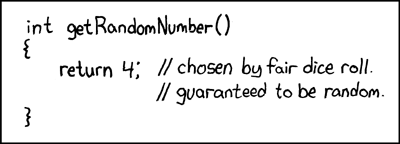
\includegraphics[width=0.6\textwidth]{images/random_number.png} \\

Credit: Randall Monroe, xkcd.com
\end{center}

\end{frame}

\begin{frame}
\begin{center}
\Large
Introduction to JAGS
\end{center}
\end{frame}


\begin{frame}
\frametitle{Introduction to JAGS}

\begin{itemize}
\item JAGS is a general purpose computer program for doing
MCMC sampling.\pause
\item It is useful for routine analyses (less useful for very large or
research problems).\pause
\item You tell it the prior, the sampling distribution, and the data and it will
do everything for you!\pause
\item It uses methods other than Metropolis (Gibbs sampling,
slice sampling, ...).
\end{itemize}

\end{frame}


\begin{frame}
\frametitle{Alternatives to JAGS}

There are some other programs similar to JAGS. I will mention them here,
so that you've heard of them, but we will not use them in this course.

\begin{itemize}
\item WinBUGS and OpenBUGS are both very similar to JAGS (the former is very
old and only works on Microsoft Windows).
Most of the time, code would not need to be modified to work in any of these.\pause
\item {\bf Stan} is a more modern and very popular package. It uses similar
ideas to JAGS, but its language is a bit different, and it uses a different,
more complex
MCMC sampler (based on {\bf Hamiltonian Monte Carlo}).
\end{itemize}

\end{frame}

\begin{frame}[fragile]
\frametitle{Installing JAGS}
You can install JAGS by first downloading it from this URL. Install it to
the default location on your system to avoid problems later.

\begin{center}
\url{https://mcmc-jags.sourceforge.io/}
\end{center}

\pause

After installing JAGS itself, you should install the \mintinline{r}{rjags}
package inside R:
\begin{minted}{r}
install.packages("rjags")
\end{minted}

\end{frame}


\end{document}

